Nas tabelas, estão marcadas em vermelho as características que os manipuladores
não preencheram, em relação aos requisitos do processo HVOF ou às restrições do
ambiente e logística, de acordo com o acesso em estudo. Em amarelo, são
assinalados os manipuladores que cumpriram com as principais caracterísiticas,
mas ainda não cumprem as exigências da solução conceitual, sendo necessária
alguma alteração no manipulador. Em verde, são assinalados os manipuladores que
cumprem todas as exigências e estão pronto para o uso.
 
\section{Acesso pela escotilha inferior - estudo de
mercado}\label{ape::bighatch}
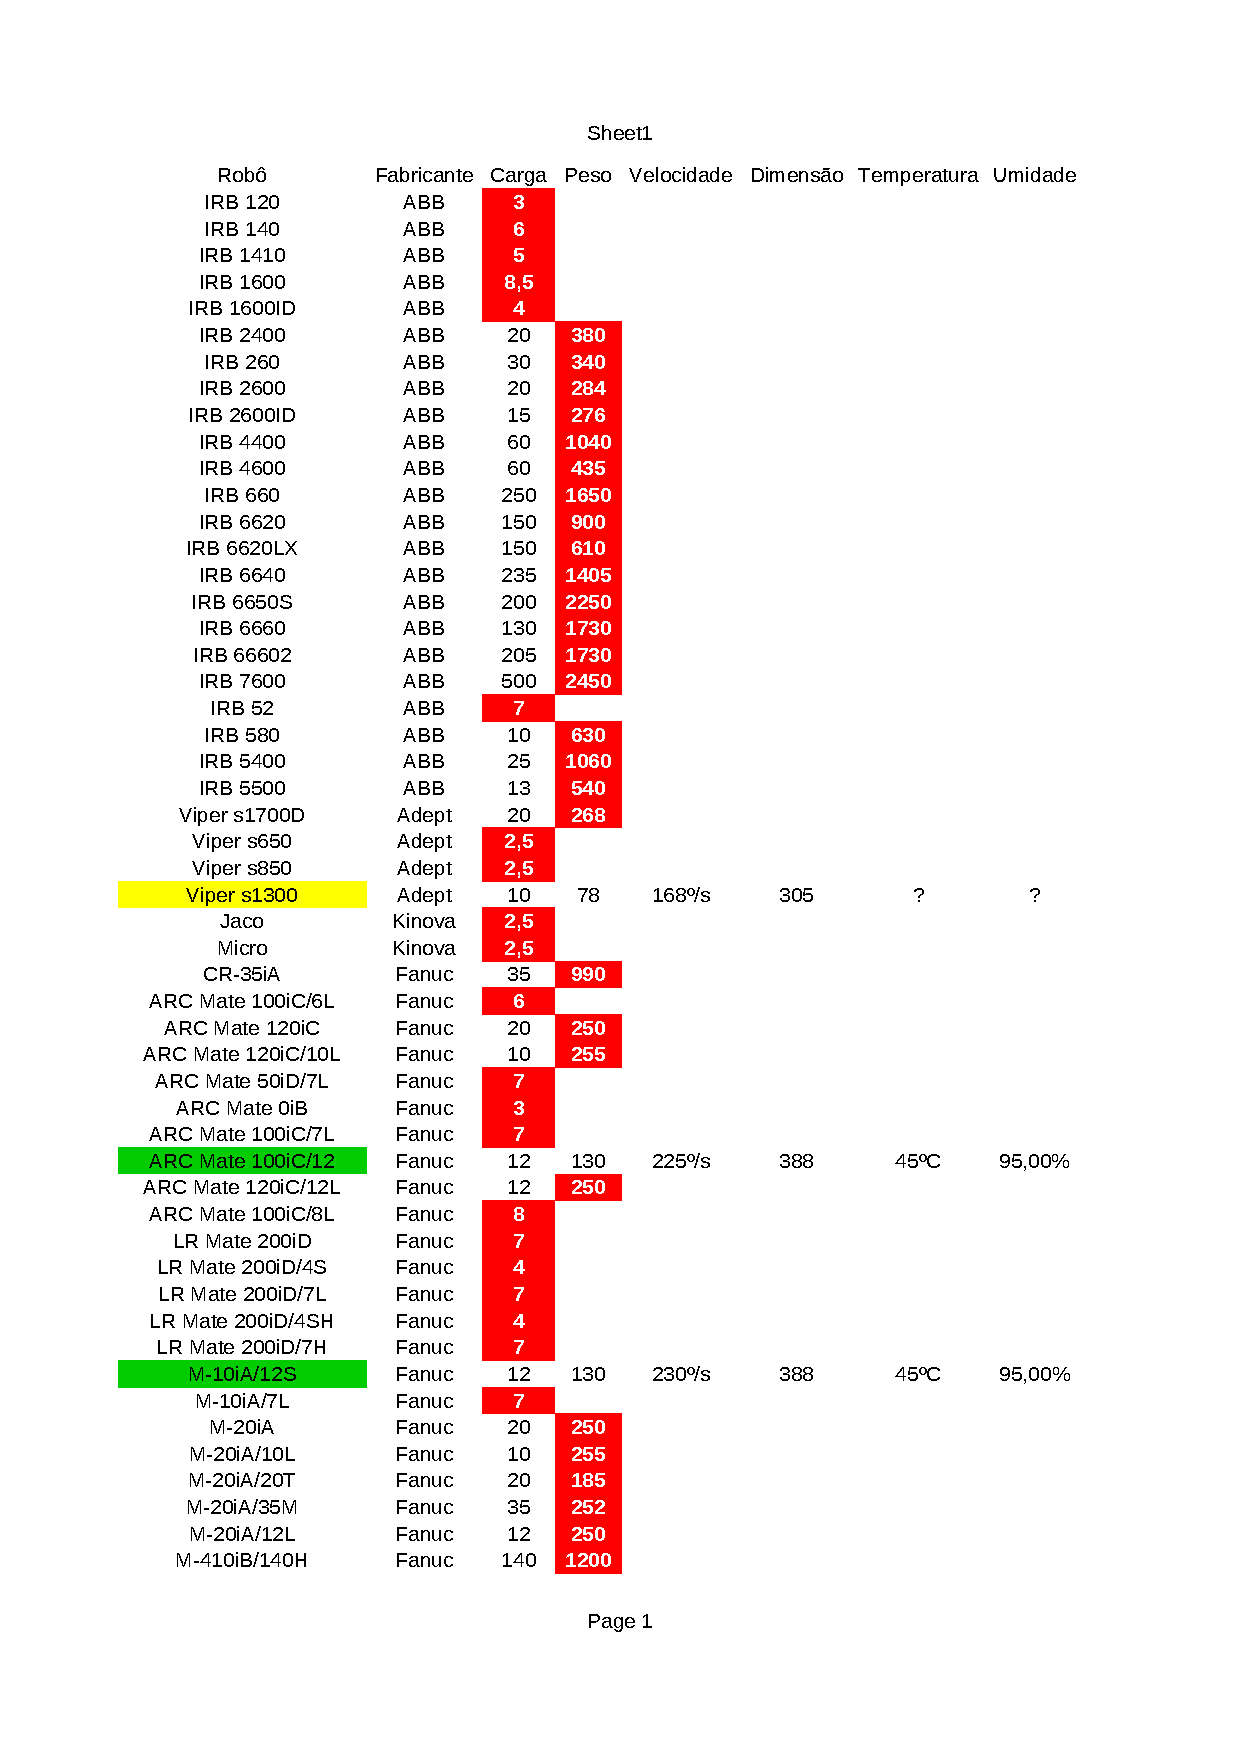
\includepdf[pages=1-]{detail/Apendice/marketbighatch}

